\section{Interface}

\begin{figure}[H]
    \centering
    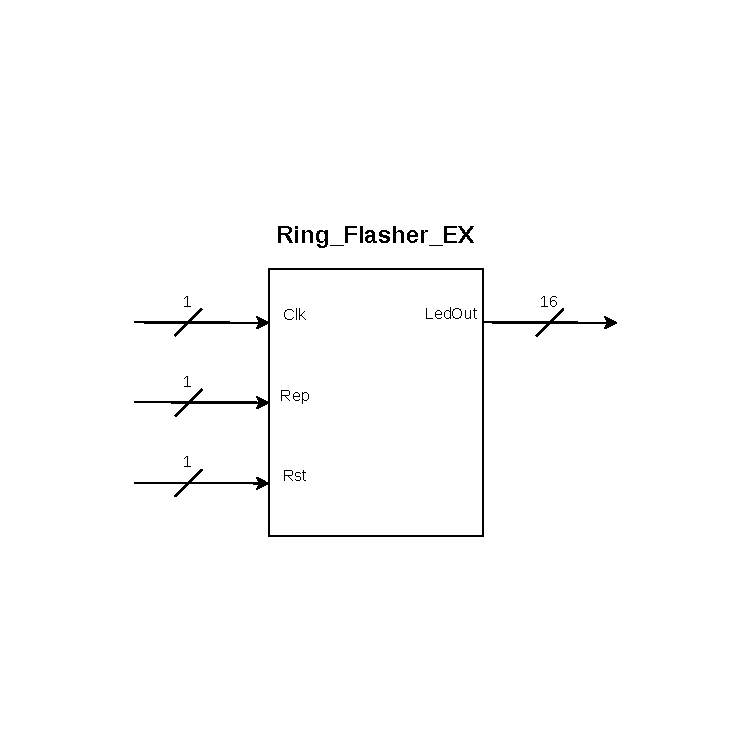
\includegraphics[width=1\linewidth]{graphics/Interface_lab1.pdf}
    \caption{The interface of the Ring Flasher module.}
    \label{tab:interface_ring_flasher}
\end{figure}

\begin{table}[H]
\centering
\caption{Interface of Ring\_Flasher\_EX}
\begin{tabular}{|c|c|c|c|}
\hline
\textbf{Signal} & \textbf{In/Out} & \textbf{Width} & \textbf{Description} \\ \hline
Clk    & Input  & 1  & System clock signal \\ \hline
Rep    & Input  & 1  & Control signal to repeat the LED pattern \\ \hline
Rst    & Input  & 1  & Reset signal (active high) \\ \hline
LedOut & Output & 16 & Output signal driving 16 LEDs \\ \hline
\end{tabular}
\end{table}